\section{Visualisation} \label{visualisation}

Figure \ref{fig:visualisation} shows two pictures of the the animation available at the end of the computation, for the former and the new software. The improvements are the following: 
\begin{itemize}
	\item The former program only showed the targets surveyed by an actuator. Now, every targets are shown.
	\item As mentioned in Section \ref{fiber_attribution}, each target are set on one of the three fibers available. IR targets are shown in orange, Visible ones in red and Calibration ones in pink. Any target's color change requires hardcoding, however the operation is straightforward; the code to change is given in Appendix 5.
	\item Actuators have also been colorised depending on their functions, respecting the color code on Figures \ref{fig:reminder:sloan_arrangement} and \ref{fig:sloan:arrangement} : empty one are transparent, fiducial ones are red, those with an IR fiber are in blue while the others are in green.
\end{itemize}

\begin{figure}[h]
\begin{center}
	\begin{subfigure}{0.9\textwidth}
		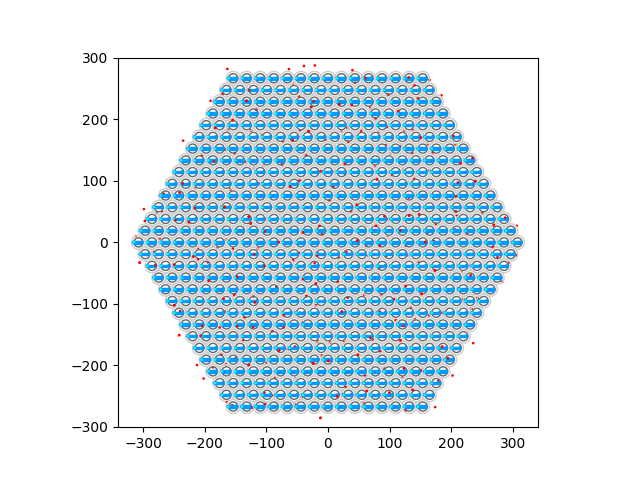
\includegraphics[width=0.9\textwidth]{visualisation/former.png}
		\caption{Former animation picture.}
		\label{fig:visualisation:former}
	\end{subfigure}
	\begin{subfigure}{0.9\textwidth}
		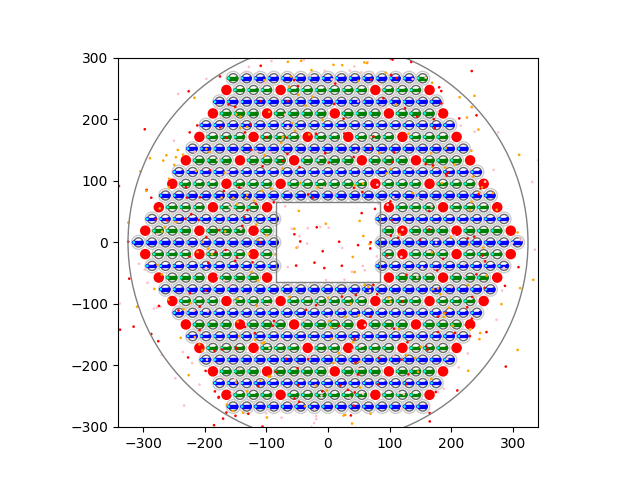
\includegraphics[width=0.9\textwidth]{visualisation/new.png}
		\caption{New animation picture.}
		\label{fig:visualisation:new}
	\end{subfigure}
	\caption{Former and new pictures of the animation available at the end of the computation. Explanations are given in Section \ref{visualisation}.}
	\label{fig:visualisation}
\end{center}
\end{figure}